% Fig. 3.9 -- 三個變數依序遞增所對應的區域: 單位立方體之中的一個四面體。
% 書稿來源: mathstatch3.tex 第 990 行的 tikzpicture (scale=.7)。
%
% 幾何一律照書稿: view={320}{345}、三軸標 $x_1$、$x_2$、$x_3$、z 軸軸名旋轉 -90 度、
% 三軸刻度都是 0、0.5、1；四面體的頂點為 (0,0,0)、(0,0,1)、(0,1,1) 與 (1,1,1)，
% 由四個 \fill 各畫一面組成；三條實線畫立方體靠前的稜邊，
% 四條虛線畫 (x,x,x)、(0,x,x)、(x,1,1) 與 (x,x,1)。
%
% 對書稿的四處調整:
%   1. 填色由 gray 0.2 改為 journalaccent 0.15；虛線改 journalmuted 0.5pt、
%      實線與座標軸改 journalink 0.8pt。
%   2. 書稿以 scale=.7 縮整張圖而字級不隨之縮，換算下來下標只有 4.9pt，
%      在 309px 顯示寬之下不到 9px。本圖改為不縮圖、直接指定 axis 的 width，
%      並以 \DeclareMathSizes 把 script 級撐到 9pt。
%   3. 書稿末尾那道 \addplot3[surf, samples=30, opacity=0] 只用來決定 x 與 y 的
%      軸範圍，本身不顯示，轉檔卻會留下約九百條看不見的路徑。本圖改以
%      xmin/xmax/ymin/ymax 直接指定範圍並加 enlargelimits=false，成圖相同。
%   4. 本圖置於 Example 方框之內，手機顯示寬為 309px 而非 350px，字級依 309px 核算。
%
% 量測: viewBox 寬 216.67pt，309px 之下放大 1.4261 倍，最小字 9pt 折合 12.83px
%       (350px 之下為 14.54px)。成圖 14 KB，gzip 之後 4.4 KB，路徑 41 條。
%
% 產製 (CH3 規格 3.2 的 pgfplots 路徑，-O 不可省):
%   latex -interaction=nonstopmode '\def\pgfsysdriver{pgfsys-dvisvgm.def}% Fig. 3.9 -- 三個變數依序遞增所對應的區域: 單位立方體之中的一個四面體。
% 書稿來源: mathstatch3.tex 第 990 行的 tikzpicture (scale=.7)。
%
% 幾何一律照書稿: view={320}{345}、三軸標 $x_1$、$x_2$、$x_3$、z 軸軸名旋轉 -90 度、
% 三軸刻度都是 0、0.5、1；四面體的頂點為 (0,0,0)、(0,0,1)、(0,1,1) 與 (1,1,1)，
% 由四個 \fill 各畫一面組成；三條實線畫立方體靠前的稜邊，
% 四條虛線畫 (x,x,x)、(0,x,x)、(x,1,1) 與 (x,x,1)。
%
% 對書稿的四處調整:
%   1. 填色由 gray 0.2 改為 journalaccent 0.15；虛線改 journalmuted 0.5pt、
%      實線與座標軸改 journalink 0.8pt。
%   2. 書稿以 scale=.7 縮整張圖而字級不隨之縮，換算下來下標只有 4.9pt，
%      在 309px 顯示寬之下不到 9px。本圖改為不縮圖、直接指定 axis 的 width，
%      並以 \DeclareMathSizes 把 script 級撐到 9pt。
%   3. 書稿末尾那道 \addplot3[surf, samples=30, opacity=0] 只用來決定 x 與 y 的
%      軸範圍，本身不顯示，轉檔卻會留下約九百條看不見的路徑。本圖改以
%      xmin/xmax/ymin/ymax 直接指定範圍並加 enlargelimits=false，成圖相同。
%   4. 本圖置於 Example 方框之內，手機顯示寬為 309px 而非 350px，字級依 309px 核算。
%
% 量測: viewBox 寬 216.67pt，309px 之下放大 1.4261 倍，最小字 9pt 折合 12.83px
%       (350px 之下為 14.54px)。成圖 14 KB，gzip 之後 4.4 KB，路徑 41 條。
%
% 產製 (CH3 規格 3.2 的 pgfplots 路徑，-O 不可省):
%   latex -interaction=nonstopmode '\def\pgfsysdriver{pgfsys-dvisvgm.def}% Fig. 3.9 -- 三個變數依序遞增所對應的區域: 單位立方體之中的一個四面體。
% 書稿來源: mathstatch3.tex 第 990 行的 tikzpicture (scale=.7)。
%
% 幾何一律照書稿: view={320}{345}、三軸標 $x_1$、$x_2$、$x_3$、z 軸軸名旋轉 -90 度、
% 三軸刻度都是 0、0.5、1；四面體的頂點為 (0,0,0)、(0,0,1)、(0,1,1) 與 (1,1,1)，
% 由四個 \fill 各畫一面組成；三條實線畫立方體靠前的稜邊，
% 四條虛線畫 (x,x,x)、(0,x,x)、(x,1,1) 與 (x,x,1)。
%
% 對書稿的四處調整:
%   1. 填色由 gray 0.2 改為 journalaccent 0.15；虛線改 journalmuted 0.5pt、
%      實線與座標軸改 journalink 0.8pt。
%   2. 書稿以 scale=.7 縮整張圖而字級不隨之縮，換算下來下標只有 4.9pt，
%      在 309px 顯示寬之下不到 9px。本圖改為不縮圖、直接指定 axis 的 width，
%      並以 \DeclareMathSizes 把 script 級撐到 9pt。
%   3. 書稿末尾那道 \addplot3[surf, samples=30, opacity=0] 只用來決定 x 與 y 的
%      軸範圍，本身不顯示，轉檔卻會留下約九百條看不見的路徑。本圖改以
%      xmin/xmax/ymin/ymax 直接指定範圍並加 enlargelimits=false，成圖相同。
%   4. 本圖置於 Example 方框之內，手機顯示寬為 309px 而非 350px，字級依 309px 核算。
%
% 量測: viewBox 寬 216.67pt，309px 之下放大 1.4261 倍，最小字 9pt 折合 12.83px
%       (350px 之下為 14.54px)。成圖 14 KB，gzip 之後 4.4 KB，路徑 41 條。
%
% 產製 (CH3 規格 3.2 的 pgfplots 路徑，-O 不可省):
%   latex -interaction=nonstopmode '\def\pgfsysdriver{pgfsys-dvisvgm.def}% Fig. 3.9 -- 三個變數依序遞增所對應的區域: 單位立方體之中的一個四面體。
% 書稿來源: mathstatch3.tex 第 990 行的 tikzpicture (scale=.7)。
%
% 幾何一律照書稿: view={320}{345}、三軸標 $x_1$、$x_2$、$x_3$、z 軸軸名旋轉 -90 度、
% 三軸刻度都是 0、0.5、1；四面體的頂點為 (0,0,0)、(0,0,1)、(0,1,1) 與 (1,1,1)，
% 由四個 \fill 各畫一面組成；三條實線畫立方體靠前的稜邊，
% 四條虛線畫 (x,x,x)、(0,x,x)、(x,1,1) 與 (x,x,1)。
%
% 對書稿的四處調整:
%   1. 填色由 gray 0.2 改為 journalaccent 0.15；虛線改 journalmuted 0.5pt、
%      實線與座標軸改 journalink 0.8pt。
%   2. 書稿以 scale=.7 縮整張圖而字級不隨之縮，換算下來下標只有 4.9pt，
%      在 309px 顯示寬之下不到 9px。本圖改為不縮圖、直接指定 axis 的 width，
%      並以 \DeclareMathSizes 把 script 級撐到 9pt。
%   3. 書稿末尾那道 \addplot3[surf, samples=30, opacity=0] 只用來決定 x 與 y 的
%      軸範圍，本身不顯示，轉檔卻會留下約九百條看不見的路徑。本圖改以
%      xmin/xmax/ymin/ymax 直接指定範圍並加 enlargelimits=false，成圖相同。
%   4. 本圖置於 Example 方框之內，手機顯示寬為 309px 而非 350px，字級依 309px 核算。
%
% 量測: viewBox 寬 216.67pt，309px 之下放大 1.4261 倍，最小字 9pt 折合 12.83px
%       (350px 之下為 14.54px)。成圖 14 KB，gzip 之後 4.4 KB，路徑 41 條。
%
% 產製 (CH3 規格 3.2 的 pgfplots 路徑，-O 不可省):
%   latex -interaction=nonstopmode '\def\pgfsysdriver{pgfsys-dvisvgm.def}\input{three-uniform-region-a.tex}'
%   dvisvgm -O -d2 -n -o ../../images/teaching-topics/three-uniform-region-a.svg three-uniform-region-a.dvi

\documentclass[tikz,border=2pt]{standalone}
\usepackage{amsmath}
\usepackage{amssymb}
\usepackage{xcolor}
\usepackage{pgfplots}
\pgfplotsset{compat=1.18}

\definecolor{journalink}{HTML}{1F1C18}
\definecolor{journalmuted}{HTML}{8A7F72}
\definecolor{journalaccent}{HTML}{9C2D2D}

%% 三個軸名的下標一律撐到 9pt。
\DeclareMathSizes{10}{10}{9}{8}

\begin{document}
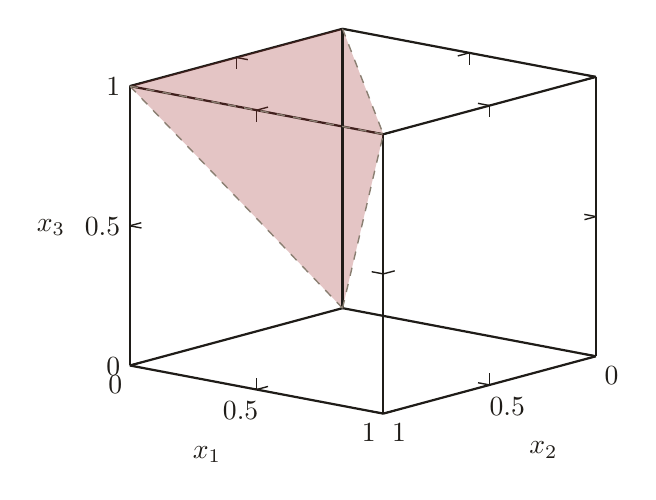
\begin{tikzpicture}
\begin{axis}[
    width=7.5cm,
    view={320}{345},
    xlabel=$x_1$,
    ylabel={$x_2$},
    zlabel={$x_3$},
    zlabel style={rotate=-90, anchor=east},
    label style={journalink},
    tick label style={journalink},
    axis line style={journalink, line width=0.8pt},
    every tick/.style={journalink, line width=0.5pt},
    enlargelimits=false,
    xmin=0, xmax=1,
    ymin=0, ymax=1,
    zmin=0, zmax=1,
    xtick={0,0.5,1},
    ytick={0,0.5,1},
    ztick={0,0.5,1},
]

%% 四面體的四個面
\fill[journalaccent, fill opacity=0.15]
  (axis cs: 0,0,0) -- (axis cs: 0,0,1) -- (axis cs: 0,1,1) -- cycle;
\fill[journalaccent, fill opacity=0.15]
  (axis cs: 0,0,0) -- (axis cs: 0,0,1) -- (axis cs: 1,1,1) -- cycle;
\fill[journalaccent, fill opacity=0.15]
  (axis cs: 0,0,0) -- (axis cs: 0,1,1) -- (axis cs: 1,1,1) -- cycle;
\fill[journalaccent, fill opacity=0.15]
  (axis cs: 0,0,1) -- (axis cs: 0,1,1) -- (axis cs: 1,1,1) -- cycle;

%% 立方體靠前的三條稜邊
\addplot3 [journalink, line width=0.8pt, domain=0:1, samples y=1, smooth] (0, 0, x);
\addplot3 [journalink, line width=0.8pt, domain=0:1, samples y=1, smooth] (0, x, 0);
\addplot3 [journalink, line width=0.8pt, domain=0:1, samples y=1, smooth] (x, 0, 0);

%% 四條輔助虛線
\addplot3 [journalmuted, line width=0.5pt, dashed, domain=0:1, samples y=1, smooth] (x, x, x);
\addplot3 [journalmuted, line width=0.5pt, dashed, domain=0:1, samples y=1, smooth] (0, x, x);
\addplot3 [journalmuted, line width=0.5pt, dashed, domain=0:1, samples y=1, smooth] (x, 1, 1);
\addplot3 [journalmuted, line width=0.5pt, dashed, domain=0:1, samples y=1, smooth] (x, x, 1);

\end{axis}
\end{tikzpicture}
\end{document}
'
%   dvisvgm -O -d2 -n -o ../../images/teaching-topics/three-uniform-region-a.svg three-uniform-region-a.dvi

\documentclass[tikz,border=2pt]{standalone}
\usepackage{amsmath}
\usepackage{amssymb}
\usepackage{xcolor}
\usepackage{pgfplots}
\pgfplotsset{compat=1.18}

\definecolor{journalink}{HTML}{1F1C18}
\definecolor{journalmuted}{HTML}{8A7F72}
\definecolor{journalaccent}{HTML}{9C2D2D}

%% 三個軸名的下標一律撐到 9pt。
\DeclareMathSizes{10}{10}{9}{8}

\begin{document}
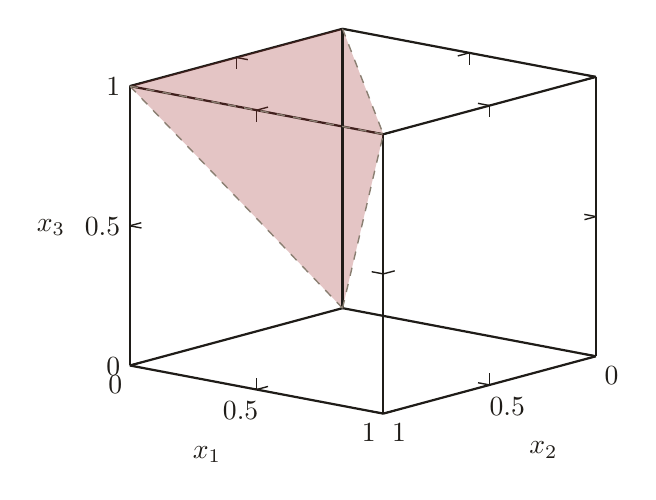
\begin{tikzpicture}
\begin{axis}[
    width=7.5cm,
    view={320}{345},
    xlabel=$x_1$,
    ylabel={$x_2$},
    zlabel={$x_3$},
    zlabel style={rotate=-90, anchor=east},
    label style={journalink},
    tick label style={journalink},
    axis line style={journalink, line width=0.8pt},
    every tick/.style={journalink, line width=0.5pt},
    enlargelimits=false,
    xmin=0, xmax=1,
    ymin=0, ymax=1,
    zmin=0, zmax=1,
    xtick={0,0.5,1},
    ytick={0,0.5,1},
    ztick={0,0.5,1},
]

%% 四面體的四個面
\fill[journalaccent, fill opacity=0.15]
  (axis cs: 0,0,0) -- (axis cs: 0,0,1) -- (axis cs: 0,1,1) -- cycle;
\fill[journalaccent, fill opacity=0.15]
  (axis cs: 0,0,0) -- (axis cs: 0,0,1) -- (axis cs: 1,1,1) -- cycle;
\fill[journalaccent, fill opacity=0.15]
  (axis cs: 0,0,0) -- (axis cs: 0,1,1) -- (axis cs: 1,1,1) -- cycle;
\fill[journalaccent, fill opacity=0.15]
  (axis cs: 0,0,1) -- (axis cs: 0,1,1) -- (axis cs: 1,1,1) -- cycle;

%% 立方體靠前的三條稜邊
\addplot3 [journalink, line width=0.8pt, domain=0:1, samples y=1, smooth] (0, 0, x);
\addplot3 [journalink, line width=0.8pt, domain=0:1, samples y=1, smooth] (0, x, 0);
\addplot3 [journalink, line width=0.8pt, domain=0:1, samples y=1, smooth] (x, 0, 0);

%% 四條輔助虛線
\addplot3 [journalmuted, line width=0.5pt, dashed, domain=0:1, samples y=1, smooth] (x, x, x);
\addplot3 [journalmuted, line width=0.5pt, dashed, domain=0:1, samples y=1, smooth] (0, x, x);
\addplot3 [journalmuted, line width=0.5pt, dashed, domain=0:1, samples y=1, smooth] (x, 1, 1);
\addplot3 [journalmuted, line width=0.5pt, dashed, domain=0:1, samples y=1, smooth] (x, x, 1);

\end{axis}
\end{tikzpicture}
\end{document}
'
%   dvisvgm -O -d2 -n -o ../../images/teaching-topics/three-uniform-region-a.svg three-uniform-region-a.dvi

\documentclass[tikz,border=2pt]{standalone}
\usepackage{amsmath}
\usepackage{amssymb}
\usepackage{xcolor}
\usepackage{pgfplots}
\pgfplotsset{compat=1.18}

\definecolor{journalink}{HTML}{1F1C18}
\definecolor{journalmuted}{HTML}{8A7F72}
\definecolor{journalaccent}{HTML}{9C2D2D}

%% 三個軸名的下標一律撐到 9pt。
\DeclareMathSizes{10}{10}{9}{8}

\begin{document}
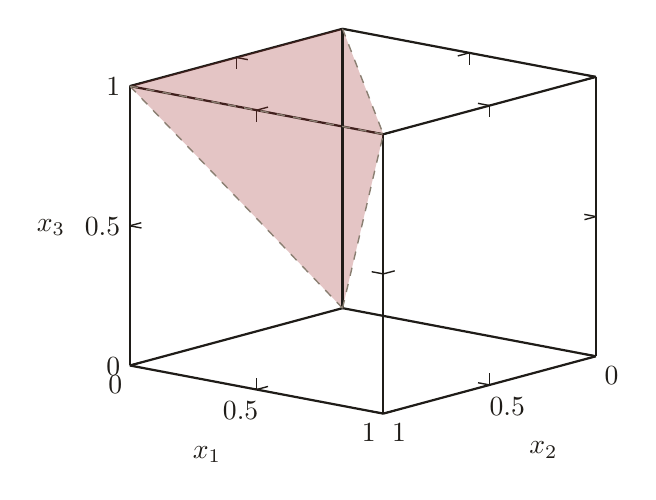
\begin{tikzpicture}
\begin{axis}[
    width=7.5cm,
    view={320}{345},
    xlabel=$x_1$,
    ylabel={$x_2$},
    zlabel={$x_3$},
    zlabel style={rotate=-90, anchor=east},
    label style={journalink},
    tick label style={journalink},
    axis line style={journalink, line width=0.8pt},
    every tick/.style={journalink, line width=0.5pt},
    enlargelimits=false,
    xmin=0, xmax=1,
    ymin=0, ymax=1,
    zmin=0, zmax=1,
    xtick={0,0.5,1},
    ytick={0,0.5,1},
    ztick={0,0.5,1},
]

%% 四面體的四個面
\fill[journalaccent, fill opacity=0.15]
  (axis cs: 0,0,0) -- (axis cs: 0,0,1) -- (axis cs: 0,1,1) -- cycle;
\fill[journalaccent, fill opacity=0.15]
  (axis cs: 0,0,0) -- (axis cs: 0,0,1) -- (axis cs: 1,1,1) -- cycle;
\fill[journalaccent, fill opacity=0.15]
  (axis cs: 0,0,0) -- (axis cs: 0,1,1) -- (axis cs: 1,1,1) -- cycle;
\fill[journalaccent, fill opacity=0.15]
  (axis cs: 0,0,1) -- (axis cs: 0,1,1) -- (axis cs: 1,1,1) -- cycle;

%% 立方體靠前的三條稜邊
\addplot3 [journalink, line width=0.8pt, domain=0:1, samples y=1, smooth] (0, 0, x);
\addplot3 [journalink, line width=0.8pt, domain=0:1, samples y=1, smooth] (0, x, 0);
\addplot3 [journalink, line width=0.8pt, domain=0:1, samples y=1, smooth] (x, 0, 0);

%% 四條輔助虛線
\addplot3 [journalmuted, line width=0.5pt, dashed, domain=0:1, samples y=1, smooth] (x, x, x);
\addplot3 [journalmuted, line width=0.5pt, dashed, domain=0:1, samples y=1, smooth] (0, x, x);
\addplot3 [journalmuted, line width=0.5pt, dashed, domain=0:1, samples y=1, smooth] (x, 1, 1);
\addplot3 [journalmuted, line width=0.5pt, dashed, domain=0:1, samples y=1, smooth] (x, x, 1);

\end{axis}
\end{tikzpicture}
\end{document}
'
%   dvisvgm -O -d2 -n -o ../../images/teaching-topics/three-uniform-region-a.svg three-uniform-region-a.dvi

\documentclass[tikz,border=2pt]{standalone}
\usepackage{amsmath}
\usepackage{amssymb}
\usepackage{xcolor}
\usepackage{pgfplots}
\pgfplotsset{compat=1.18}

\definecolor{journalink}{HTML}{1F1C18}
\definecolor{journalmuted}{HTML}{8A7F72}
\definecolor{journalaccent}{HTML}{9C2D2D}

%% 三個軸名的下標一律撐到 9pt。
\DeclareMathSizes{10}{10}{9}{8}

\begin{document}
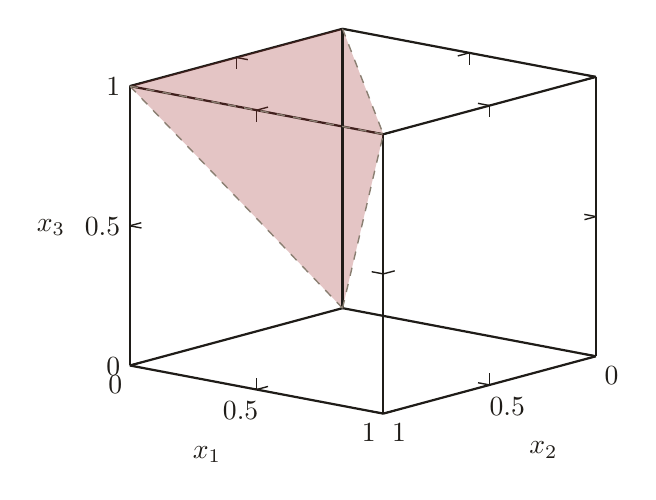
\begin{tikzpicture}
\begin{axis}[
    width=7.5cm,
    view={320}{345},
    xlabel=$x_1$,
    ylabel={$x_2$},
    zlabel={$x_3$},
    zlabel style={rotate=-90, anchor=east},
    label style={journalink},
    tick label style={journalink},
    axis line style={journalink, line width=0.8pt},
    every tick/.style={journalink, line width=0.5pt},
    enlargelimits=false,
    xmin=0, xmax=1,
    ymin=0, ymax=1,
    zmin=0, zmax=1,
    xtick={0,0.5,1},
    ytick={0,0.5,1},
    ztick={0,0.5,1},
]

%% 四面體的四個面
\fill[journalaccent, fill opacity=0.15]
  (axis cs: 0,0,0) -- (axis cs: 0,0,1) -- (axis cs: 0,1,1) -- cycle;
\fill[journalaccent, fill opacity=0.15]
  (axis cs: 0,0,0) -- (axis cs: 0,0,1) -- (axis cs: 1,1,1) -- cycle;
\fill[journalaccent, fill opacity=0.15]
  (axis cs: 0,0,0) -- (axis cs: 0,1,1) -- (axis cs: 1,1,1) -- cycle;
\fill[journalaccent, fill opacity=0.15]
  (axis cs: 0,0,1) -- (axis cs: 0,1,1) -- (axis cs: 1,1,1) -- cycle;

%% 立方體靠前的三條稜邊
\addplot3 [journalink, line width=0.8pt, domain=0:1, samples y=1, smooth] (0, 0, x);
\addplot3 [journalink, line width=0.8pt, domain=0:1, samples y=1, smooth] (0, x, 0);
\addplot3 [journalink, line width=0.8pt, domain=0:1, samples y=1, smooth] (x, 0, 0);

%% 四條輔助虛線
\addplot3 [journalmuted, line width=0.5pt, dashed, domain=0:1, samples y=1, smooth] (x, x, x);
\addplot3 [journalmuted, line width=0.5pt, dashed, domain=0:1, samples y=1, smooth] (0, x, x);
\addplot3 [journalmuted, line width=0.5pt, dashed, domain=0:1, samples y=1, smooth] (x, 1, 1);
\addplot3 [journalmuted, line width=0.5pt, dashed, domain=0:1, samples y=1, smooth] (x, x, 1);

\end{axis}
\end{tikzpicture}
\end{document}
